\documentclass{llncs}
%
%
%espero que no se enfaden por incluir este paquete:
\usepackage{amsmath}
\usepackage{amssymb}
%\usepackage{amsthm}

\usepackage[dvips]{graphicx}
\usepackage{makeidx}  % allows for indexgeneration
\usepackage{color}
\usepackage[table]{xcolor}

\hyphenation{pro-per-ties}
\hyphenation{ge-ne-ral-ly}
\hyphenation{pre-fe-ren-ces}
\hyphenation{u-sing}
\hyphenation{pu-nish-ment}
\newcommand{\Pow}{\mathcal{P}}
\newcommand{\N}{\operatorname{N}}
\newcommand{\bool}{\operatorname*{\mathcal{B}}}
\newcommand{\Pos}{\operatorname{Pos}}
\newcommand{\Nec}{\operatorname{Nec}}
\newcommand{\Open}{\operatorname{Open}}
\newcommand{\Rp}{\operatorname{Rp}}
\newcommand{\Rn}{\operatorname{Rn}}
\newcommand{\FB}{\operatorname{FB}}
\newcommand{\UC}{\operatorname{UC}}
\newcommand{\T}{\mathcal{T}}
\newcommand{\Rel}{\mathcal{R}}
\newcommand{\C}{\mathcal{C}}
\newcommand{\Nat}{\mathbb{N}}
\newcommand{\Boolean}{\mathbb{B}}
\newcommand{\Q}{\mathbb{Q}}
\newcommand{\R}{\mathbb{R}}
\newcommand{\Z}{\mathbb{Z}}
\newcommand{\Head}{\mathcal{H}}
\newcommand{\Body}{\mathcal{B}}
\newcommand{\Dom}{\mathcal{D}}
\newcommand{\INS}{\mbox{\textbf{insert}}}
\newcommand{\DEL}{\mbox{\textbf{delete}}}
\newcommand{\MOD}{\mbox{\textbf{modify}}}
\newcommand{\REV}{\mbox{\textbf{revise}}}
\newcommand{\Overlap}{\mbox{\textbf{Overlap}}}
\newcommand{\A}{\mathcal{A}}
\newcommand{\I}{\mathcal{I}}
\renewcommand{\Join}{\bowtie}
%\theoremstyle{definition}
%\newtheorem{definition}{Definition}
\begin{document}

\mainmatter              % start of the contributions
%
\title{Evaluation of the Allen's relations for two Possibilistic Time Periods.}
%
%\titlerunning{A Fuzzy Valid-Time Model}  % abbreviated title (for running head)
%                                     also used for the TOC unless
%                                     \toctitle is used
%
\author{
%Jos\'e Enrique Pons
 }
%Jeffrey Dean \and David Grove \and Craig Chambers \and Kim~B.~Bruce \and
%Elsa Bertino}
%
\authorrunning{Jos\'e Enrique Pons et al.} % abbreviated author list (for running head)
%
%%%% list of authors for the TOC (use if author list has to be modified)
%\tocauthor{Ivar Ekeland, Roger Temam, Jeffrey Dean, David Grove,
%Craig Chambers, Kim B. Bruce, and Elisa Bertino}
%
\institute{
% Department of Computer Science and Artificial Intelligence \\
% Universidad de Granada \\
% Escuela T\'ecnica Superior de Ingenier\'ia Inform\'atica \\
% C/Periodista Daniel Saucedo Aranda s/n \\
% E-18071 (Granada-Spain)\\
% \email{jpons,opc@decsai.ugr.es}\\ 
%WWW home page:
%\texttt{http://users/\homedir iekeland/web/welcome.html}
%\and
%Universit\'{e} de Paris-Sud,
%Laboratoire d'Analyse Num\'{e}rique, B\^{a}timent 425,\\
%F-91405 Orsay Cedex, France
}

\maketitle              % typeset the title of the contribution

\begin{abstract}

\end{abstract}

\section{\label{sec:intro}Introduction}
In this work we propose the evaluation of the Allen's relations for time intervals for two given possibilistic time periods.


\section{\label{sec:implementation}Implementation of the Allen's Relations}

In the following we will consider a possibilistic time interval (\emph{PTI}) be $I = \left[S_i, E_i \right]$. Where $S_i$ and $E_i$ are possibilistic time points representing the starting and the ending boundaries of the time interval.

Each possibilistic time point is given by $P = \left[D, a, b \right]$. This notation represents that:
\begin{itemize}
 \item $D$ is the central main point.
\item $D-a$ is the left point.
\item $D+b$ is the right point.
\end{itemize}
 
In the following, a time interval $I$ will be noted as:
\begin{align}
 I = \left[S_i, E_i \right]\\
S_i = \left[D_{S_i},a_{S_i},b_{S_i} \right] \\
E_i = \left[D_{E_i},a_{E_i},b_{E_i} \right]
\end{align}

% The following proposal translates an interval end-points constraint to several ill-known constraints that allows the evaluation for two pvps.

A relation between two crisp time points $m, n$ is given by the following expression.
\begin{equation}
\label{eq:general-crisp-comparison}
\left(n\  R \  m \right) 
\end{equation}
Where  $R$ is one of the following: $\left \lbrace <, >, \leq, \geq, = \right \rbrace$.
The result of the expression is a boolean value indicating whether the point $n$ is in the relation $\left( R, m \right)$.

\begin{equation}
\label{eq:boolean-crisp-comparison}
n \in A:\left(a, m \right) \in R
\end{equation}

% A crisp constraint can be translated to a set of two ill-known constraint. First of all, the end-points $a, b$ are in the possibilistic case to two ill-known time points: $A_i, B_j$
% \begin{equation}
%  \left( =, A_i \right) \wedge \left(R, B_j \right)
% \end{equation}
\subsection{\label{subsec:translation}Translation to the possibilistic case}
In order to implement the Allen's relations for two possibilistic valid-time periods, we need to translate the expression in \eqref{eq:general-crisp-comparison} to the possibilistic case. In this case, we will note \eqref{eq:general-crisp-comparison} as the following:

\begin{equation}
\label{eq:general-possibilistic-comparison}
\left(P_n\  R \  P_m \right) 
\end{equation}

Where:
\begin{itemize}
 \item  $P_n$ is either the starting or ending point of the possibilistic time interval given by $I = \left[S_i, E_i \right]$.
\item $P_m$ is either the starting or ending point of the possibilistic time interval given by $J = \left[S_j, E_j \right]$.
\item $R \in \left \lbrace <, >, \leq, \geq, = \right \rbrace$.
\end{itemize}

The evaluation of the expression \eqref{eq:general-possibilistic-comparison} is equivalent to the following ill-known constraints:
\begin{align}
 \label{eq:evaluation-by-ill-known}
\left(P_n\  R \  P_m \right)  &\triangleq \lambda \left( C_1 , C_2 \right) \\
\nonumber
& C_1 =\left(=, P_n \right) \\
\nonumber
& C_2 = \left(R, P_m \right)
\end{align}

Consider that $a \in A \subseteq U$, then:
\begin{align}
 \label{eq:evaluation-1}
\Pos \left(C_1 \left(A \right)\right) &= \min_{a  \in A} \left(\pi_{P_n} \left(a \right) \right)\\
\nonumber
\Nec \left(C_1 \left(A \right) \right) &= \min_{a  \in A} \left(1-\pi_{P_n} \left(a \right)\right)\\
\nonumber
\Pos \left(C_2 \left(A \right)\right) &= \min_{a \in A} \left(\sup_{\left \lbrace a , \omega \right \rbrace \in R}  \pi_{P_m} \left(\omega \right) \right)\\
\nonumber
\Nec \left(C_2 \left(A \right) \right) &= \min_{a \in A} \left(\inf_{\left \lbrace a, \omega \right \rbrace  \not \in R} 1-\pi_{P_m}\left(\omega \right) \right)
\end{align}

With $\lambda = \left(\wedge, \left(C_1, C_2 \right) \right)$, we obtain:
\begin{align}
 \label{eq:eval-2}
\Pos \left(\lambda \left(A \right)\right) &= \max \min_{a \in A} \left(\Pos \left(C_1 \left( A\right) \right), \Pos \left(C_2\left(A \right) \right) \right)\\
\nonumber
\Nec \left(\lambda \left(A\right)\right) &= \max \min_{a \in A} \left(\Nec \left(C_1 \left( A\right) \right), \Nec \left(C_2\left(A \right) \right) \right)
\end{align}






\subsection{\label{subsec:before}Before}
The crisp version for the before operator for two crisp intervals $i = \left[s_i,e_i \right], j = \left[s_j, e_j \right]$.
\begin{equation}
i \mbox{ Before } j \triangleq \left( e_i < s_j \right)
\end{equation}
This is translated to the possibilistic case:
$I = \left[S_i, E_i \right], J = \left[S_j, E_j\right]$.

\begin{align}
 I \mbox{ Before } J &\triangleq \lambda \left(C_1, C_2 \right)\\
\nonumber
C_1 &\triangleq \left(=, E_i\right) \\
\nonumber
C_2 &\triangleq \left(<, S_j \right)
\end{align}
The possibility and the necessity of the Before relation is computed as follows:
\begin{align}
\Pos \left(\lambda \left(A \right)\right) &= \max \min_{a \in A} \left(\Pos \left(C_1 \left( A\right) \right), \Pos \left(C_2\left(A \right) \right) \right)\\
\nonumber
\Nec \left(\lambda \left(A\right)\right) &= \min \min_{a \in A} \left(\Nec \left(C_1 \left( A\right) \right), \Nec \left(C_2\left(A \right) \right) \right)
\end{align}




\begin{example}
Consider the following possibilistic time periods:
\begin{align}
I = \left( \left[1,2,2 \right] , \left[6,2,2 \right] \right)\\
\nonumber
J = \left( \left[6,1,1 \right] , \left[9,1,1 \right] \right)
\end{align}

We want to know the possibility of $I$ Before $J$. As a result of triangle's line intersection, we get:
\begin{align}
 \label{sample:before}
\Pos \left(\lambda \left(A \right)\right) &= - \frac{-D_{S_j} + D_{E_i}-a_{E_i}}{a_{S_j}+a_{E_i}}\\
\nonumber
&= - \frac{-6+6-2}{2+1} = \frac{2}{3}\\
\Nec \left(\lambda \left(A\right)\right) &= 0
\end{align}


\begin{figure}[ht]
\caption{Illustration of the before relationship.}
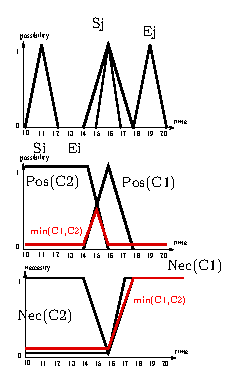
\includegraphics[scale=2.1]{./graphs/before.eps} 
\end{figure}



\end{example}







\newpage

\section*{Acknowledgements}
%
The researchers are supported by the grant BES-2009-013805 within the research project TIN2008-02066: \emph{Fuzzy Temporal Information treatment in relational DBMS}.

\bibliographystyle{splncs03}
\bibliography{biblio}




\end{document}